%@descr: wzór sprawozdania, raportu lub pracy - nadaje się do przeróbek
%@author: Maciej Komosiński

\documentclass{article} 
\usepackage{polski} 
\usepackage[utf8]{inputenc} 
\usepackage[OT4]{fontenc} 
\usepackage{graphicx,color} %include pdf's (and png's for raster graphics... avoid raster graphics!) 
\usepackage{url}
\usepackage{float}
\usepackage[pdftex,hyperfootnotes=false,pdfborder={0 0 0}]{hyperref} %za wszystkimi pakietami; pdfborder nie wszedzie tak samo zaimplementowane bo specyfikacja nieprecyzyjna; pod miktex'em po prostu nie widac wtedy ramek
\usepackage{biblatex}
\addbibresource{report.bib}

% Zmiana rozmiarów strony tekstu
\addtolength{\voffset}{-1cm}
\addtolength{\hoffset}{-1cm}
\addtolength{\textwidth}{2cm}
\addtolength{\textheight}{2cm}

%bardziej zyciowe parametry sterujace rozmieszczeniem rysunkow
\renewcommand{\topfraction}{.85}
\renewcommand{\bottomfraction}{.7}
\renewcommand{\textfraction}{.15}
\renewcommand{\floatpagefraction}{.66}
\renewcommand{\dbltopfraction}{.66}
\renewcommand{\dblfloatpagefraction}{.66}
\setcounter{topnumber}{9}
\setcounter{bottomnumber}{9}
\setcounter{totalnumber}{20}
\setcounter{dbltopnumber}{9}

% własny bullet list z malymi odstepami
\newenvironment{tightlist}{
\begin{itemize}
  \setlength{\itemsep}{1pt}
  \setlength{\parskip}{0pt}
  \setlength{\parsep}{0pt}}
{\end{itemize}}

%obrazkow szukamy w nastepujacym katalogu:
\graphicspath{{pics/}}



%\title{Sprawozdanie z laboratorium:\\Metaheurystyki i Obliczenia Inspirowane Biologicznie}
%\author{}
%\date{}


\begin{document}

\thispagestyle{empty} %bez numeru strony

\begin{center}
{\large{Sprawozdanie z laboratorium:\\
Metaheurystyki i obliczenia inspirowane biologicznie}}

\vspace{3ex}

Część I: Algorytmy optymalizacji lokalnej, problem ATSP
%Część II: Algorytmy optymalizacji lokalnej i globalnej, problem QAP
%Część III: Eksperyment: ... (prezentację można zrobić w LaTeX - służy do tego klasa "beamer")

\vspace{3ex}
{\footnotesize\today}

\end{center}


\vspace{10ex}

Prowadzący: dr hab.~inż. Maciej Komosiński

\vspace{5ex}

Autorzy:
\begin{tabular}{lllr}
    \textbf{Marcin Mrugas} & inf122580 & marcin.mrugas@student.put.poznan.pl \\
    \textbf{Piotr Kicki} & inf122401 & piotr.kicki@student.put.poznan.pl \\
\end{tabular}

\vspace{5ex}

Zajęcia środowe, 16:50.

\vspace{35ex}

\noindent Oświadczam/y, że niniejsze sprawozdanie zostało przygotowane wyłącznie przez powyższych autora/ów,
a wszystkie elementy pochodzące z innych źródeł zostały odpowiednio zaznaczone i~są cytowane w bibliografii.  

\newpage


\section*{Udział autorów}
\begin{tightlist}
\item MM zaimplementował szkielet aplikacji, przeszukiwanie losowe oraz tabu, przeprowadził eksperyment z podobieństwem, opisał ekspermenty,
\item PK zaimplementował przeszukiwanie zachłanne, lokalne oraz symulowane wyżarzanie, przeprowadził eksperyment najlepszych i średnich wyników, opisał ekspermenty.
\end{tightlist}


\section{Wstęp}

Naszym zadaniem było zaimplementowanie i przestudiowanie asymetrycznego problemu komiwojażera. Problem ten polega na znalezieniu najkrótszego cyklu Hamiltona w grafie asymetrycznym. Można go interpretować jako logistyczny problem dotyczący znalezienia takiej trasy dla dostawcy, aby ten odwiedził wszystkich odbiorców w jak najkrótszym czasie. Problem należy do klasy problemów NP-zupełnych. Złożoność tego problemu, w najgorszym przypadku, sprowadza się do przeglądnięcia wszystkich cyklów Hamiltona których dla grafu o zupełnego o $n$ wierzchołkach jest $n!$. Dlatego problem ten optymalizuje się algorytmami, które w przestrzeni rozwiązań starają się rozważać mniejszą część rozwiązań i uzyskują rozwiązania często gorsze od optymalnego, ale osiągają ten wynik w znacznie krótszym czasie.

\begin{figure}[H]
\begin{center}
    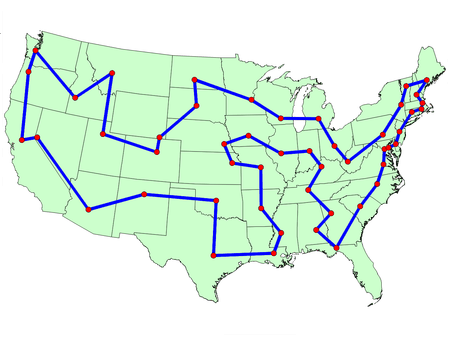
\includegraphics[width=0.6\textwidth]{map002g.png}
\end{center}
\caption{Przykładowe rozwiązanie problemu komiwojażera ze stolicami stanów Stanów Zjednoczonych Źródło: \url{http://support.sas.com/documentation/cdl/en/ornoaug/67520/HTML/default/viewer.htm}.}
\label{fig:schemat}
\end{figure}


\section{Opis sąsiedztwa}

Operatorem sąsiedztwa w naszej implementacji jest 2-OPT. Nowy sąsiad jest tworzony poprzez zamianę miejscami dwóch wierzchołków rozwiązania. 

\begin{figure} 
\begin{center}
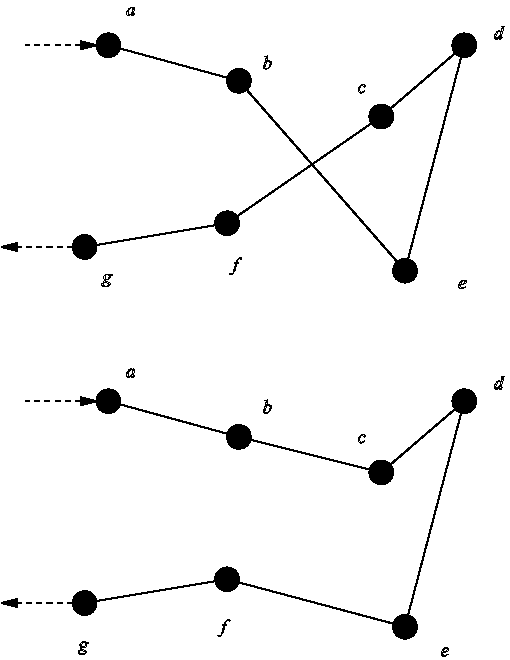
\includegraphics[width=0.4\textwidth]{twooptwiki.pdf}
\end{center}
\caption{Przykład sąsiedztwa.}
\label{fig:schemat2}
\end{figure}


\section{Opis algorytmów}

Pominiemy opis trywialnych algorytmów jak LS, H-nearest oraz RS, aby skupić się na TS oraz SA.

Działanie Tabu Search przebiega następująco. Na początku algorytm losuje rozwiązanie startowe po czym w każdej iteracji wybiera 1000 losowych sąsiadów i liczy dla każdego z nich deltę, aby stworzyć master listę. Następnie ta lista jest sortowana rosnąco po obliczonych deltach. W kolejnym kroku lista jest przeglądana od najlepszych ruchów do najgorszych i zmiany zostają wprowadzone w tymczasowym rozwiązaniu. Jadnak jest możliwe że nie wszystkie ruchy zostaną wykorzystane. Zależy to od listy tabu, która przechowuje informacje ile iteracji temu wybrany ruch został użyty. Lista jest aktualizowana za każdym razem kiedy zostanie wprowadzona zmiana i jeżeli jakiś ruch został wcześniej wykorzystany nie jest on aplikowany. Kadencja w naszej implementacji trwa 15 iteracji. Aby odblokować ruchy pod koniec każdej iteracji lista tabu jest dekrementowana. Na końcu rozwiązanie tymczasowe jest zapisywane jeżeli jest krótsze od dotychczas najlepszego. Algorytm kończy się gdy przez 100 iteracji nie uzyska poprawy.


Algorytm Simulated Annealing na samym początku określa temperature startową poprzez wylosowanie $K$ rozwiązań, sprawdzeniu całego sąsiedztwa oraz zapisaniu uzyskanych delt. $K$ w naszej implementacji wynosiło $\frac{100 * N^2}{2}$, gdzie $N$ to rozmiar instancji. Następnie dla delt które dawały gorsze rozwiązanie jest liczona średnia wartość różnicy jakości $\Delta_{avg}$ oraz stosunek -- $ratio$ gorszych sąsiadów, czy takich dla których różnica jakiości była mniejsza od zera, do wszystkich przejrzanych. Wtedy temperatura początkowa jest obliczana jako:
$$
T_{start} = \frac{-\Delta_{avg}}{log((ratio - 0.15) / ratio)}
$$
Następnie zaczyna się właściwa część algorytmu. Jest losowane rozwiazanie początkowe. W każdej kolejnej iteracji jest losowany sąsiad i jeżeli jego delta $\Delta$ jest korzystna to zmiana zostaje wykorzystana, w przeciwnym przypadku jest akceptowana z prawdopodobieństwem $e^{\Delta/T}$, gdzie $T$ to aktualna temperatura. Temperatura jest aktualizowana co $N^2$ i jest obliczana z wzoru $T'=T*\alpha$, gdzie $\alpha$ to współczynnik chłodzenia i w naszej implementacji został ustawiony na wartość $0.94$.
\section{Porównanie działania algorytmów}


\subsection{Jakość}
Za miarę jakości obraliśmy wartość równania:
$$ \frac{\eta}{\eta_{min}}-1 $$
gdzie:\\
$\eta_{min}$ -- długość optimum globalnego \\
$\eta$ -- długość rozważanego rozwiązania \\
Co można interpretować jako wartość, o jaką długość rozwiązania $\eta$ jest procentowo dłuższa od rozwiązania optymalnego $\eta_{min}$.

\begin{figure}[H]
\begin{center}
    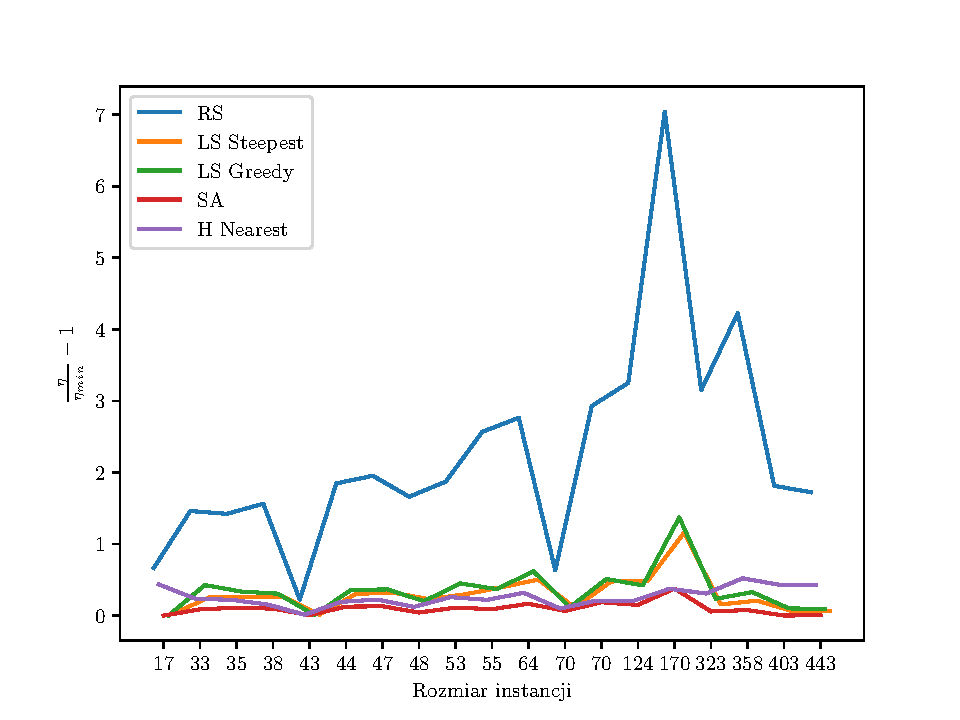
\includegraphics[width=1\textwidth]{plot_min.pdf}
\end{center}
\caption{Najlepsze uzyskane wyniki.}
\label{fig:plot_min}
\end{figure}

Na rys. \ref{fig:plot_min} przedstawiono wykres zawierający najlepsze wyniki z 10 uruchomień algorytmów. Na wykresie można zauważyć że najgorsze wyniki daje algorytm Random Search, który uzyskuje średnio jakość 1 -- 2 czyli dwukrotnie gorsze rozwiązanie od optymalnego oraz 8 razy gorsze w najgorszym przypadku. Pozostałe algorytmy osiągały zbliżoną jakość, jednakże najlepsze wyniki z nich osiągnął algorytm SA, następnie TS oraz kolejno H-nearest, LS steepest, LS greedy. Ponadto dla największych instancji algorytm heurystyczny dawał gorsze wyniki niż pozostałe algorytmy.

\begin{figure}[H]
\begin{center}
    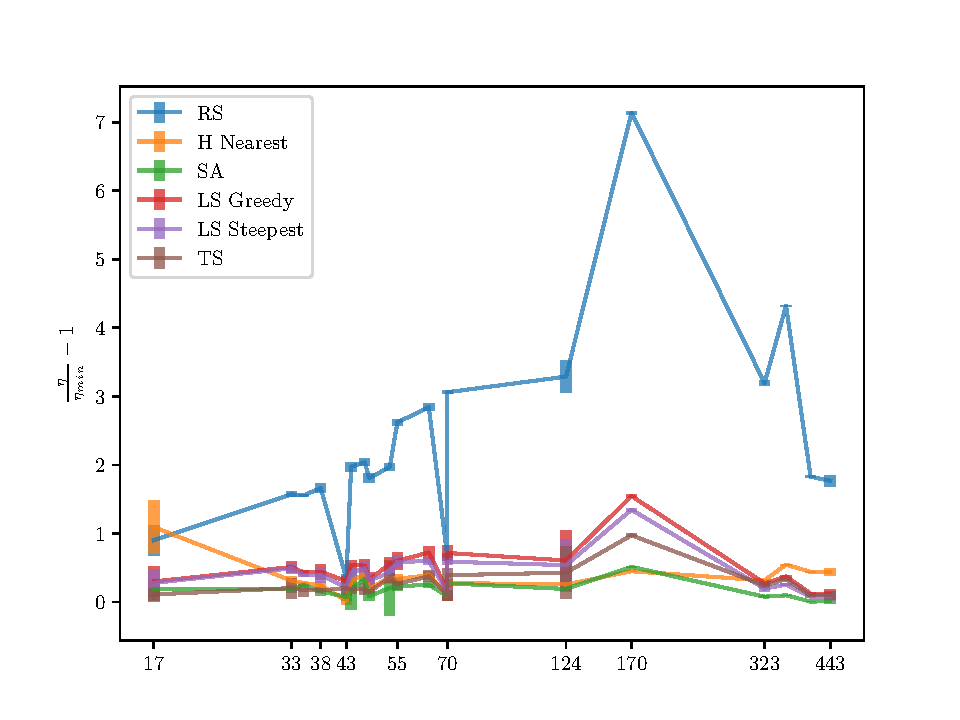
\includegraphics[width=1\textwidth]{plot_mean.pdf}
\end{center}
\caption{Średnie wyniki algorytmów}
\label{fig:plot_avg}
\end{figure}


Na rys. \ref{fig:plot_avg} zostały przedstawione średnie wyniki algorytmów. Dla czytelności rozmiary instancji są pokazane w skali logarytmicznej. Z wykresu widać, że algorytm losowy znowu dawał najgorsze wyniki, następnie algorytmy lokalne dawały lepsze wyniki i działały bardzo podobnie na korzyść algorytmu steepest. Najlepsze znowu okazały się algorytmy SA i TS. Można także zauważyć, że instancja o rozmiarze 124 charakteryzowała się dużą liczbą lokalnych optimów do których zbiegały testowane algorytmy, gdyż zaobserwowano dużą różnorodność w długości końcowych rozwiązań.

\subsection{Czas działania}

\begin{figure}[H]
\begin{center}
    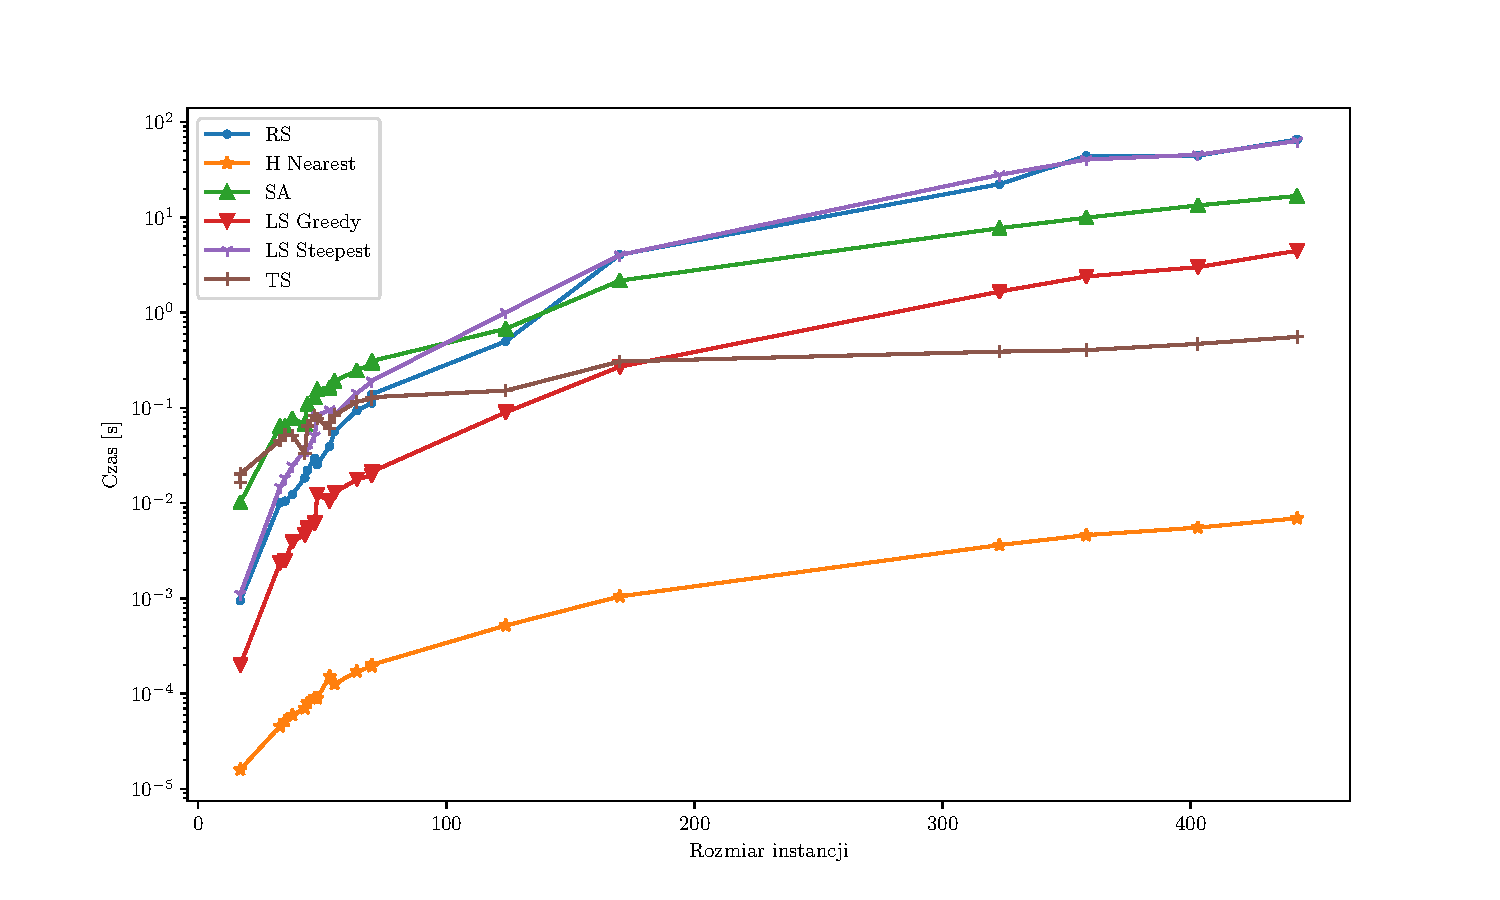
\includegraphics[width=1\textwidth]{plot_mean_time.pdf}
\end{center}
\caption{Czas działania algorytmów}
\label{fig:plot_time}
\end{figure}

Rys. \ref{fig:plot_time} Przedstawia czas działania algorytmów. Naszybciej działał algorytm heurystyczny, następnie TS, LS Greedy, SA i na końcu Steepest. Czas działania algorytmu losowego był dobrany tak aby działał porównywalnie długo jak algorytm lokalny. Widać także, że zarówno czas działania algorytmów, jak i tempo jego narastania, rośnie wraz z rozmiarem instancji. Najmniejsze tempo wzrostu można zaobserwować dla dużych instancji i algorytmu tabu, co jest pożądaną własnością.


\subsection{Efektywność}


\begin{figure}[H]
\begin{center}
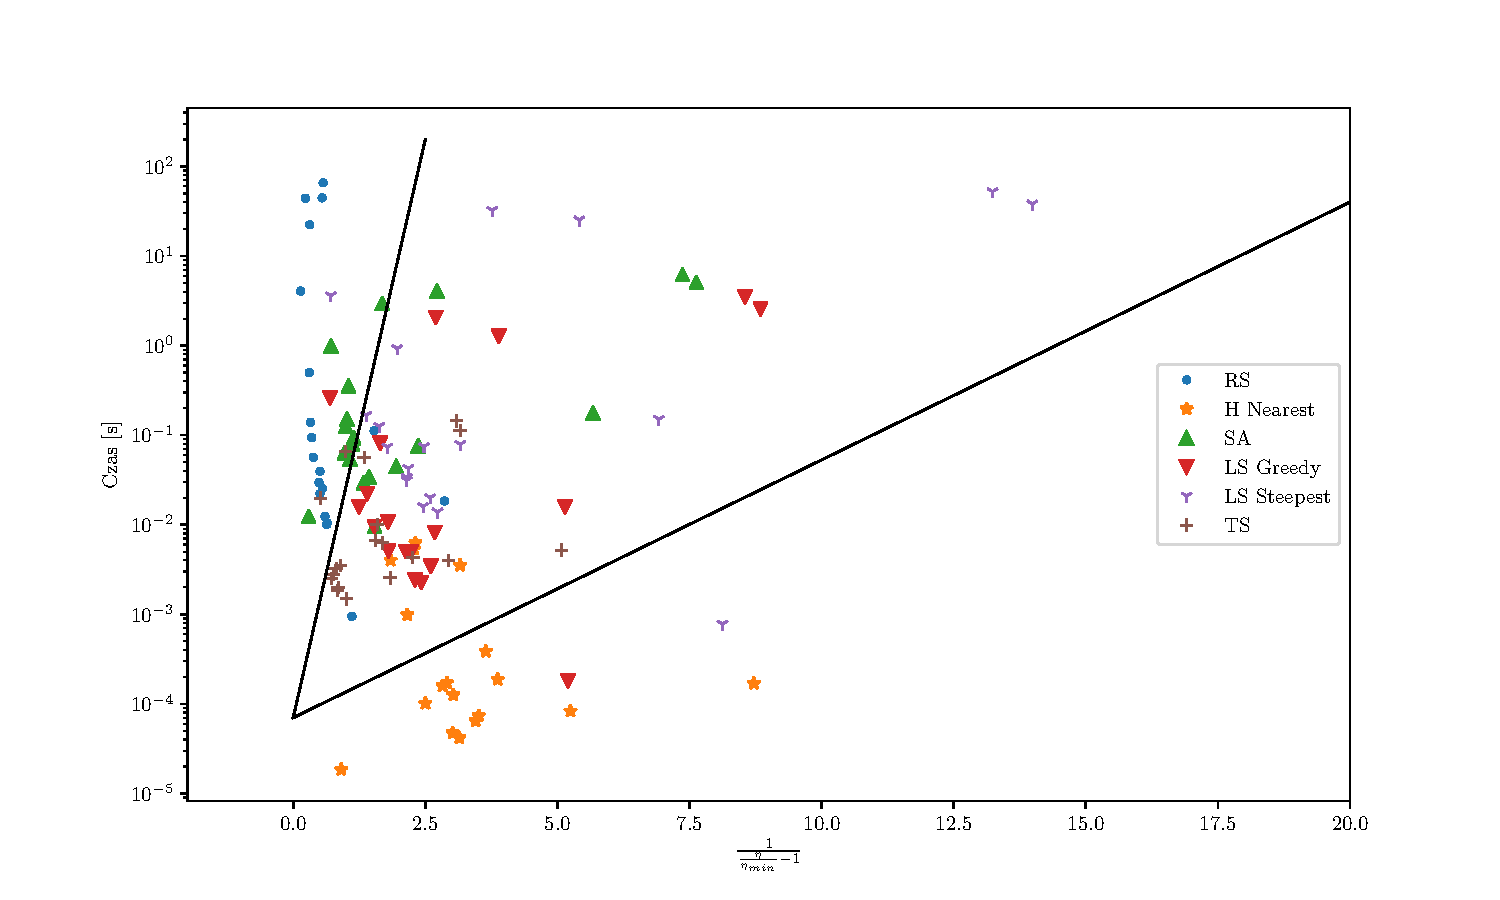
\includegraphics[width=1\textwidth]{quality.pdf}
\end{center}
\caption{Efektywność algorytmów}
\label{fig:plot_quality}
\end{figure}

Aby zbadać, który algorytm jest najbardziej efektywny biorąc pod uwagę czas działania oraz jakoś wyniku, wykreśliliśmy wykres punktowy, który przedstawia te zależności. Aby znaleźć najefektywniejsze algorytmy należy spojrzeć na kąt pomiędzy prostą łączącą początek układu współrzędnych i punktem odpowiadający instancji, a osią X. Na wykres zostały naniesione linie dzielące podobne jakościowo algorytmy. Z rys. \ref{fig:plot_quality} można wyczytać, że najlepsze wyniki w czasie uzyskał algorytm heurystyczny, a najgorsze algorytm losowy.


\subsection{Średnia liczba kroków algorytmów}

\begin{figure} 
\begin{center}
    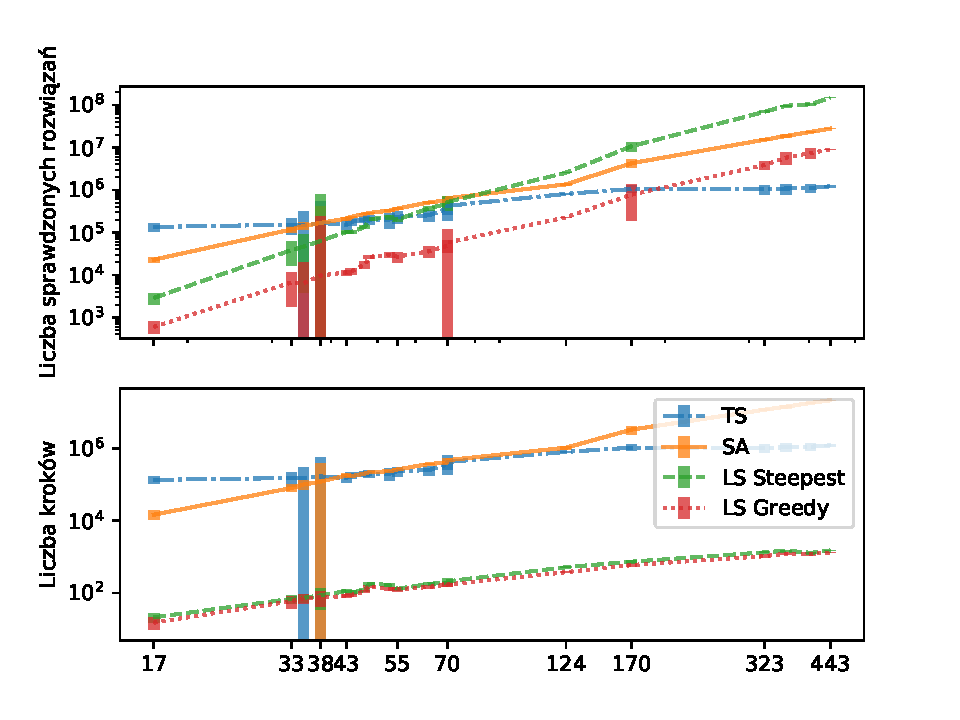
\includegraphics[width=1\textwidth]{steps.pdf}
\end{center}
\caption{(góra) Liczba sprawdzonych rozwiązań oraz (dół) liczba kroków algorytmów)}
\label{fig:plot_steps}
\end{figure}

Na rys. \ref{fig:plot_steps} przedstawiono ilość kroków i ilość ocenionych rozwiązań przez algorytmy TS, SA, Greedy i Steepest. Widać, że instancje 33 i 38 miały bardzo różne ilości sprawdzonych rozwiązań przez algorytmy. Z danych wynika także, że algorytm steepest sprawdzał najwięcej rozwiązań, zaś liczba kroków była podobna dla algorytmów LS, co może świadczyć o tym, że nie opłaca się sprawdzać wszystkich sąsiadów aby trafić w podobne minimum lokalne co algorytm Steepest, ponieważ wyniki tych algorytmów są podobne, a czas działania lepszy w algorytmie Greedy.
Algorytm SA i TS wykonywały największą liczbę kroków, jednakże SA sprawdzał znacznie więcej rozwiązań, gdyż losowo przegladał sąsiadów. Większa liczba kroków obu algorytmów świadczy o tym, że lista tabu w TS oraz temperatura w SA wychodziły z minimów lokalnych i dłużej eksplorowały przestrzeń rozwiązań.

\begin{figure}[H]
    \begin{center}
        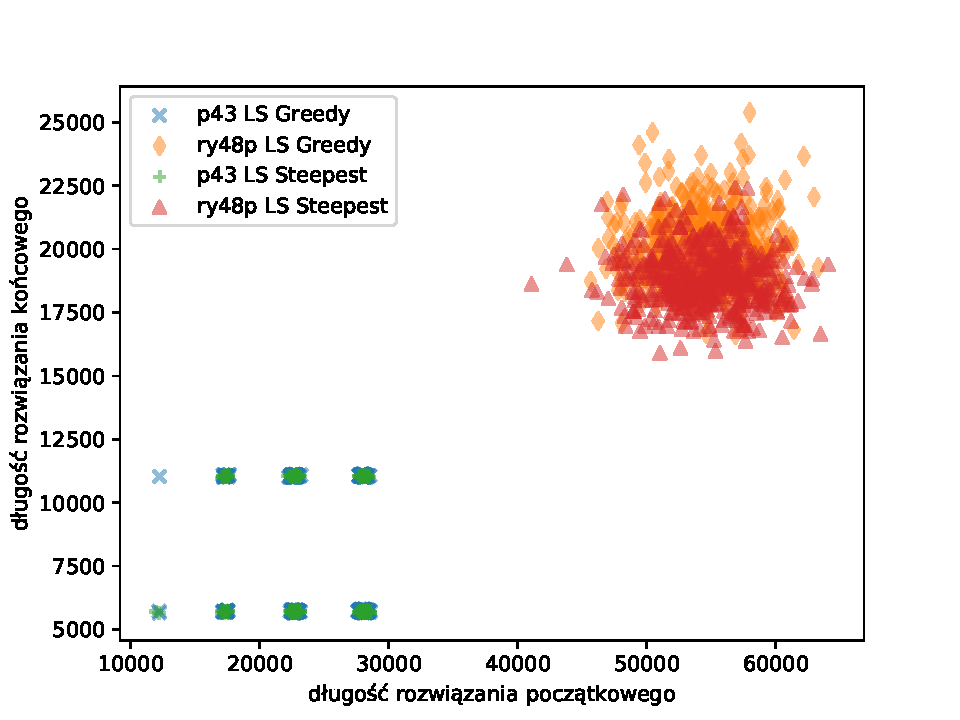
\includegraphics[width=1\textwidth]{first_last_finest.pdf}
    \end{center}
    \caption{Jakość rozwiązania początkowego, a jakość rozwiązania końcowego}
    \label{fig:first_finnest}
\end{figure}


\section{Jakość rozwiązania początkowego a jakość rozwiązania końcowego}

Rys. \ref{fig:first_finnest} przedstawia zależność długości rozwiązania początkowego i długości rozwiązania końcowego dla instancji 43 i 48. Dla instancji 248 obydwa algorytmy dawały losowe rozwiązania z tym, że algorytm steepest dawał nieco lepsze rezultaty. Dla instancji 48 oba algorytmy wpadały w podobne 4 minima lokalne i nie były wstanie polepszyć wyników. Dla tej instancji optimum lokalne miało długość 5620, co w części rozwiązań zostawało osiągane.

\section{Jakość rozwiązania w zależności od ilości uruchomień}

\begin{figure}
    \begin{center}
        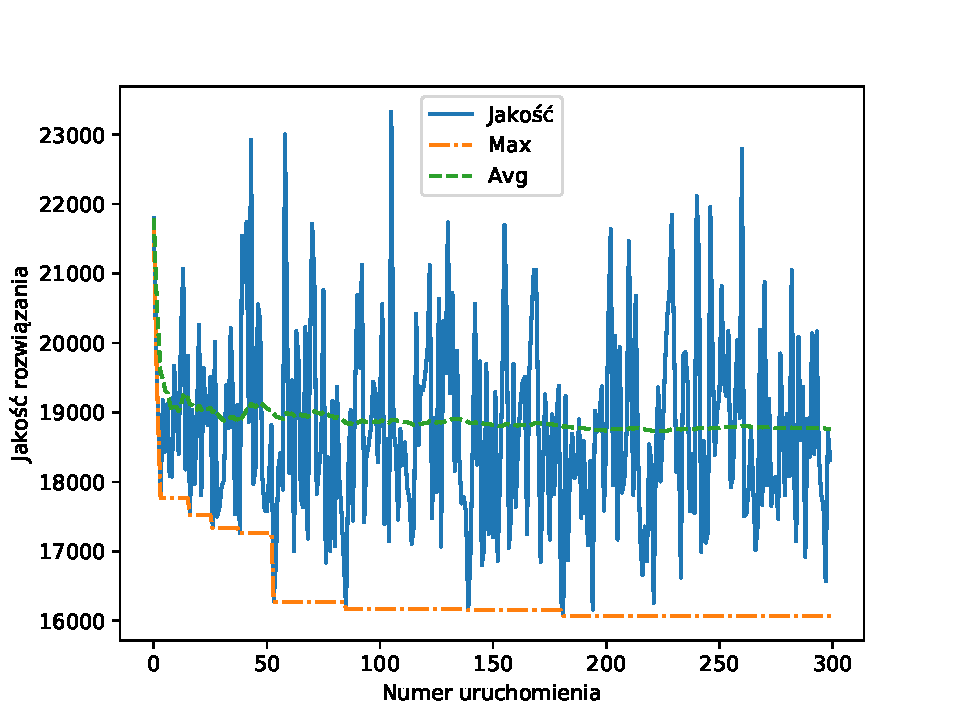
\includegraphics[width=0.9\textwidth]{multi_run_ry48p_atsp.pdf}
    \end{center}
    \caption{Jakość rozwiązania w zależności od ilości uruchomień. Instancja ry48p.}
    \label{fig:plot_multi_run_ry48p}
\end{figure}

\begin{figure}
    \begin{center}
        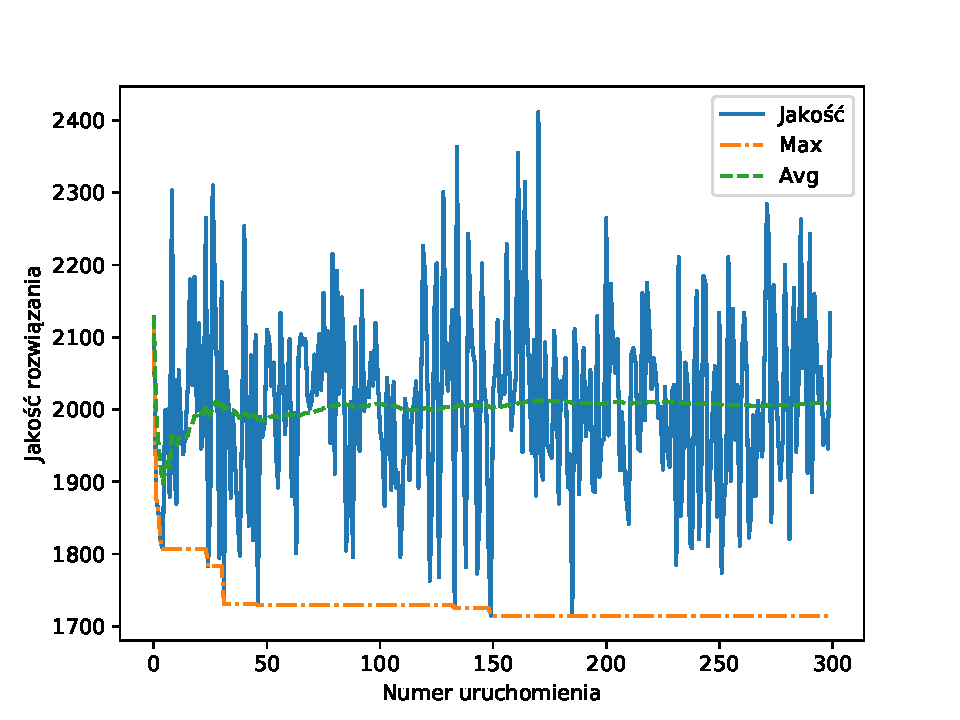
\includegraphics[width=0.9\textwidth]{multi_run_ftv35_atsp.pdf}
    \end{center}
    \caption{Jakość rozwiązania w zależności od ilości uruchomień. Instancja ftv35.}
    \label{fig:plot_multi_run_ftv35}
\end{figure}

Przedstawione na rys. \ref{fig:plot_multi_run_ry48p} i \ref{fig:plot_multi_run_ftv35}  wykresy przedstawiają jakość rozwiązania w zależności od liczby uruchomień, Z wykresów wynika że po ok 50 uruchomieniach obydwa algorytmy uzyskały drugie najlepsze wyniki spośród stu uruchomień. Na pewno można polepszyć wyniki, ale widać, że każda kolejna poprawa wymaga, co raz to większej dodatkowej ilości uruchomień. 

\section{Podobieństwo rozwiązań}

Na rys. \ref{fig:quality_sim_ftv38} i \ref{fig:quality_sim_ry48p} pokazana jest zależność pomiędzy jakością 1000 rozwiązań otrzymanych przy pomocy algorytmu Steepest, a najlepszym znalezionym optimum lokalnym. Można zauważyć, że im lepsze rozwiązanie, tym bardziej jest podobne do znalezionego optimum.

\begin{figure}
    \begin{center}
        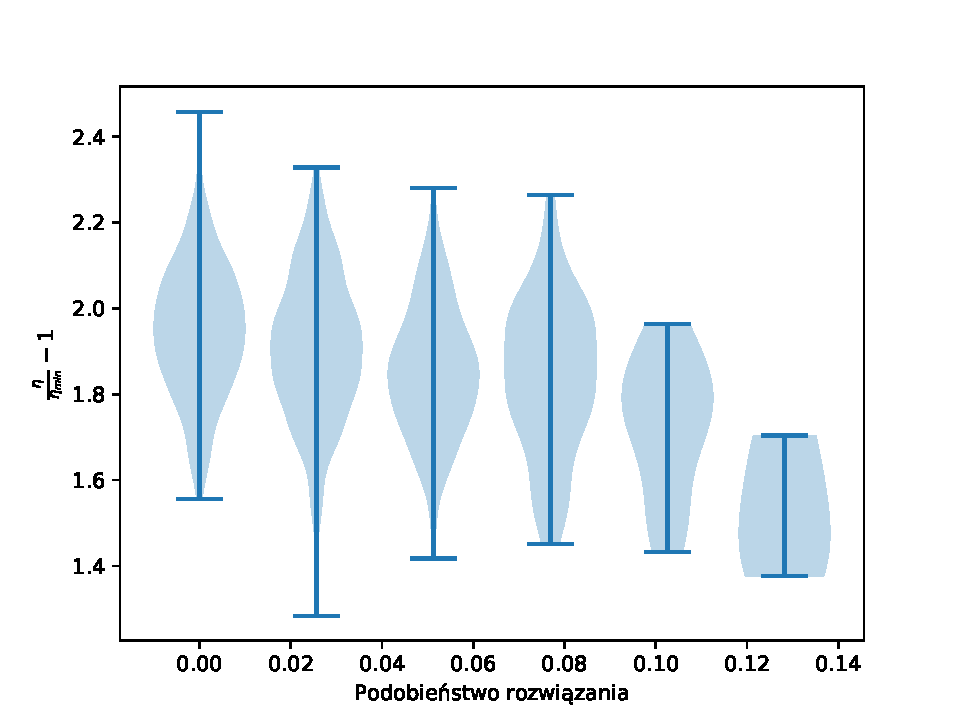
\includegraphics[width=0.8\textwidth]{quality_similarity_ftv38.pdf}
    \end{center}
    \caption{Jakość rozwiązań w zależności podobieństwa do najlepszego znalezionego optimum. Instancja ftv38.}
    \label{fig:quality_sim_ftv38}
\end{figure}

\begin{figure}
    \begin{center}
        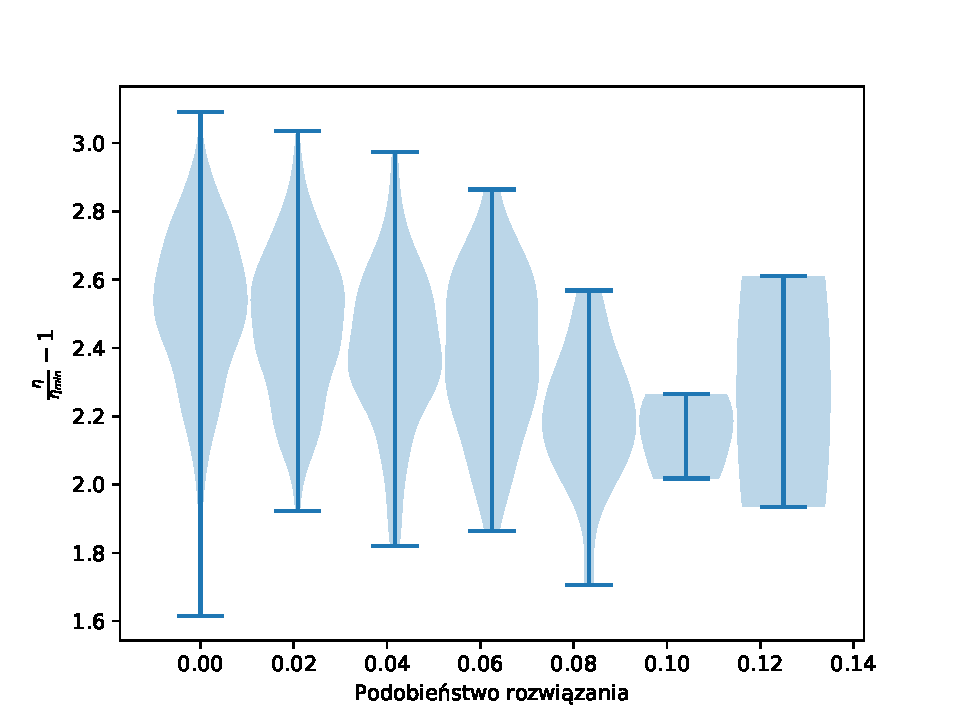
\includegraphics[width=0.8\textwidth]{quality_similarity_ry48p.pdf}
    \end{center}
    \caption{Jakość rozwiązania w zależności podobieństwa do najlepszego znalezionego optimum. Instancja ry48p.}
    \label{fig:quality_sim_ry48p}
\end{figure}


Na rys. \ref{fig:quality_sim} przedstawiono podobieństwo 15 najlepszych spośród 1000 rozwiązań oraz ich podobieństwo do najlepszego znalezionego rozwiązania. Widać ze rozwiązania różnią się a najbardziej podobne są tylko w 12.5\%.


\section{Wnioski}


Najlepsze rezultaty, zarówno jeżeli chodzi o wartość średnią, jak i minimalną, osiągał algorytm SA. Zbliżoną jakość, przy znacznie krótszym czasie działania, dla instancji małej i średniej wielkości prezentował algorytm heurystyczny. Algorytmy Greedy i Steepest osiągały zbliżone rezultaty, jednakże Steepest cechował się nieznacznie lepszą jakością rozwiązania, a Greedy czasem działania.
Najgorszą jakośc rozwiązań otrzymano dla algorytmu losowego.

\section{Trudności i problemy}

Aby wykonać poprawnie wykresy i pokazać jak najwięcej informacji trzeba poświęcić dużo czasu na ich stworzenie. Początkowo pojawiły się także problemy z budowaniem części projektu napisanej w języku C++, gdyż wymaga on narzędzi, takich jak CMake, w jednakowej wersji i konfiguracji.

\section{Propozycje udoskonaleń}

Można by jeszcze bardziej zautomatyzować wykonywanie eksperymentów i prezentację wyników (generowanie wykresów) poprzez napisanie skryptu, który kompilowałby projekt, wykonywałby wszystkie zaimplementowane eksperymenty, a nastpnie generował wykresy. Aktualnie każda z tych części jest wykonywana osobnymi poleceniami. Można było zaproponować jakąś heurystykę, w celu doboru parametrów algorytmów SA i TS.

\begin{figure}[H]
    \begin{center}
        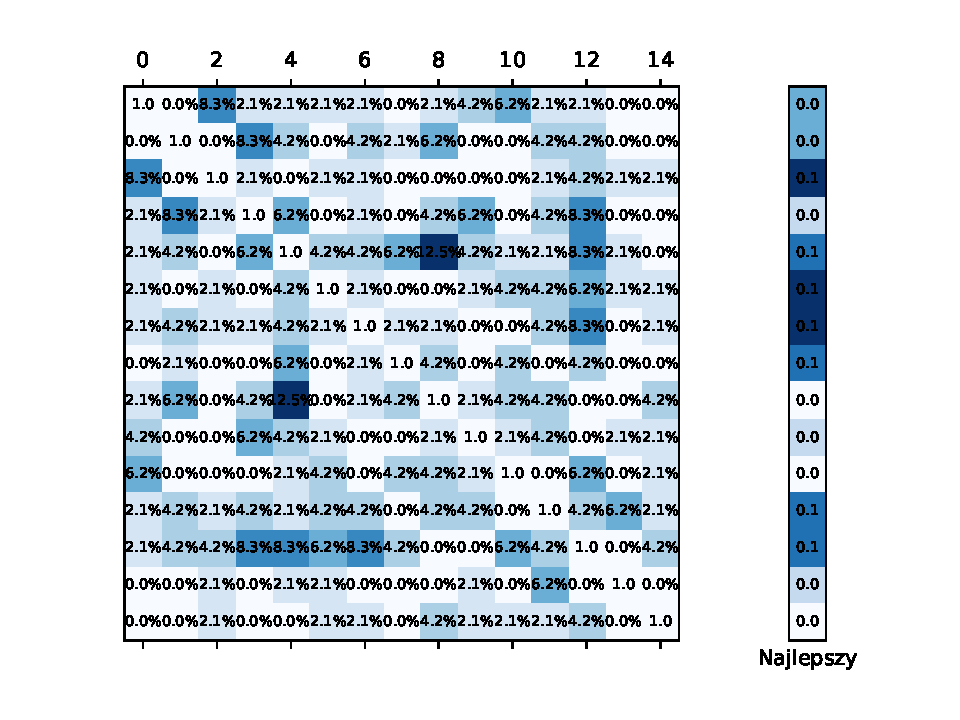
\includegraphics[width=1\textwidth]{quality_similarity_best15.pdf}
    \end{center}
    \caption{Wzajemne podobieństwo 15 najlepszych rozwiązań oraz najlepszego znalezionego optimum. Instancja ry48p.}
    \label{fig:quality_sim}
\end{figure}

\clearpage

\printbibliography


\end{document}
